\documentclass[runningheads]{llncs}
\usepackage{graphicx}
\usepackage{amsmath,amssymb} % define this before the line numbering.
\usepackage{ruler}
\usepackage{color}
\usepackage[width=122mm,left=12mm,paperwidth=146mm,height=193mm,top=12mm,paperheight=217mm]{geometry}

\usepackage{deform}

\begin{document}
% \renewcommand\thelinenumber{\color[rgb]{0.2,0.5,0.8}\normalfont\sffamily\scriptsize\arabic{linenumber}\color[rgb]{0,0,0}}
% \renewcommand\makeLineNumber {\hss\thelinenumber\ \hspace{6mm} \rlap{\hskip\textwidth\ \hspace{6.5mm}\thelinenumber}}
% \linenumbers
\pagestyle{headings}
\mainmatter
\def\ECCV12SubNumber{385}  % Insert your submission number here

\title{Supplementary Material: Learning Deformation with Parallel Transport} % Replace with your title

\titlerunning{ECCV-12 submission ID \ECCV12SubNumber}

\authorrunning{ECCV-12 submission ID \ECCV12SubNumber}

\author{Anonymous ECCV submission}
\institute{Paper ID \ECCV12SubNumber}


\maketitle
\section{Experiment Result on JAFFE database}
\label{sec:theory}
In order to illustrate additional details of our new deformation manifold with parallel transport consistency, we show figures from testing the approach on the Japanese Female Facial Expression (JAFFE) Database~\cite{JAFFE}.
The database contains 213 gray images of 7 facial expressions (6 basic facial expressions + 1 neutral) posed by 10 Japanese female models.
We randomly pick two female models, K.A. and N.M., with 23 and 20 face images repectively for our experiment and resize the image  to 128 by 128.
\subsection{Visualize Deformation Basis}
We learn a tagent space around K.A.'s neutral face from all her other images. 
We apply three different deformation operators comprised of the learned bases to her neutral face with different coefficients: the first two correspond to those with the largest eigenvalues while the third is the average of those two bases.

The first row the supplementary video shows the gradual expression deformation for all three cases with the same linearly increasing coefficient. Figure~\ref{fig:v1} shows two intermediate frames from the video.
We see that the first deformation basis learned by our model corresponds to a "sad" expression while the second basis corresponds to an "angry" expression. The third operator which has both of these two expressions creates a new blended facial expression. 
\begin{figure}[t]
    \centering
    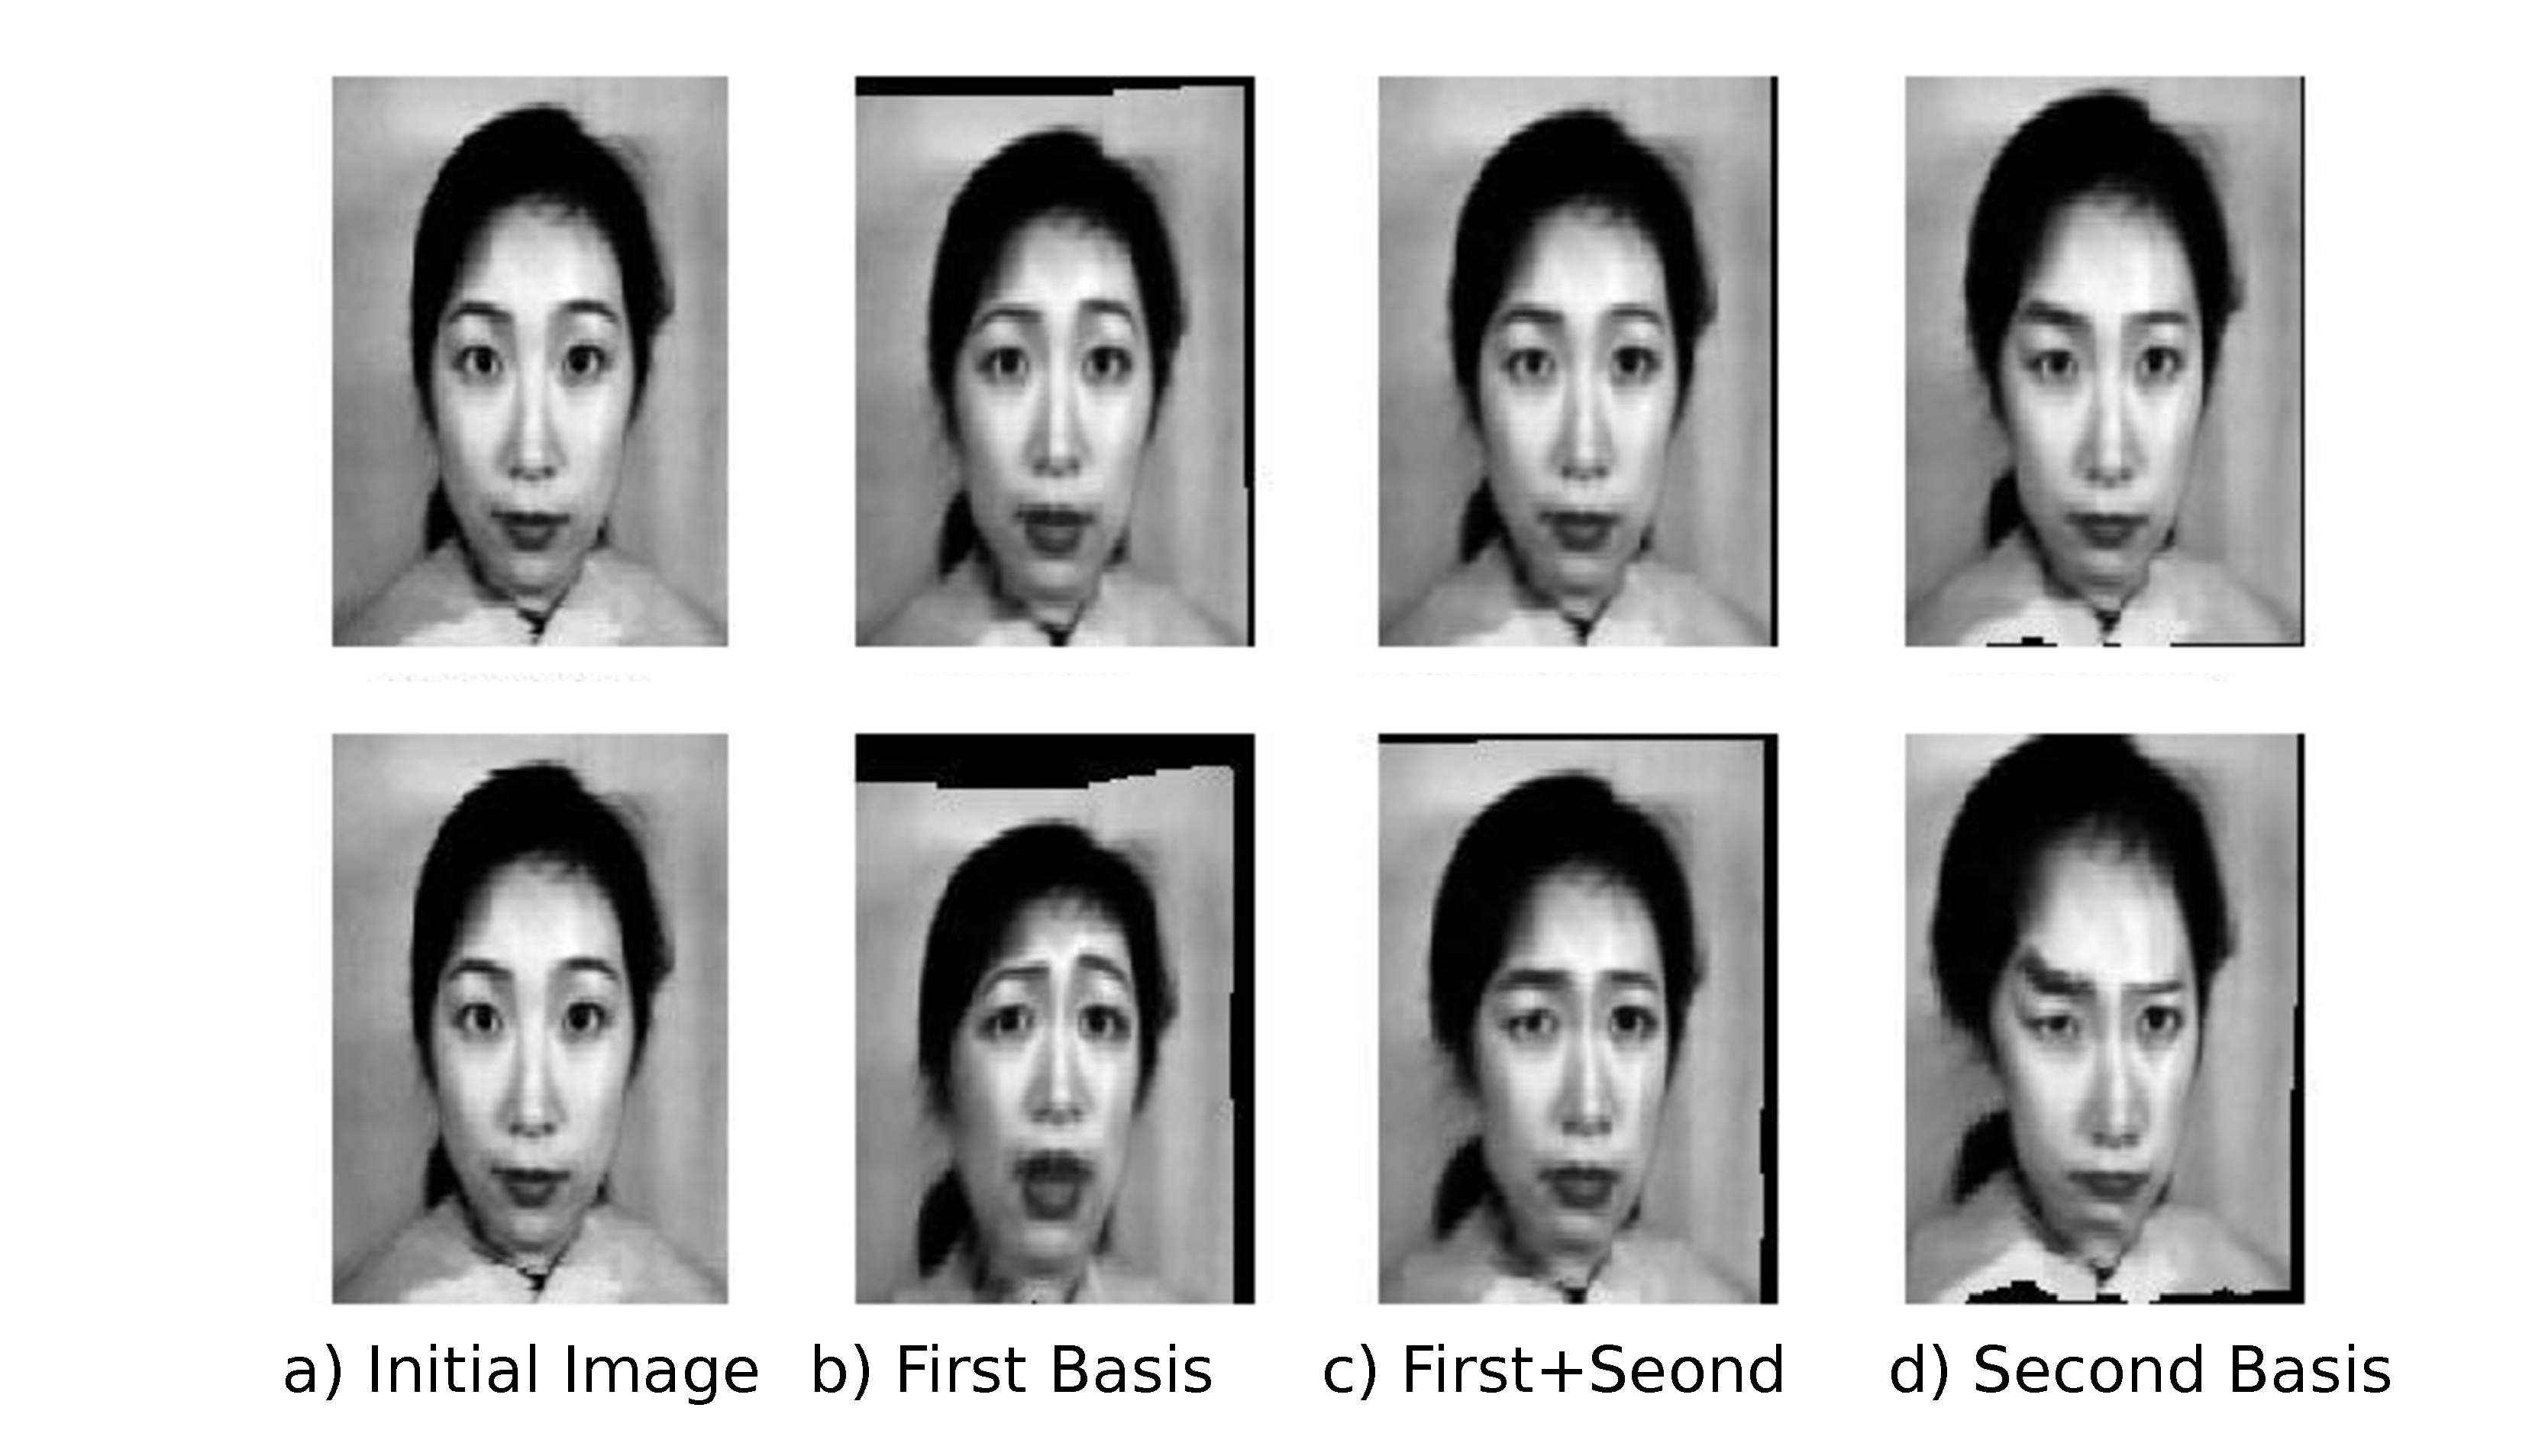
\includegraphics[height=0.6\columnwidth]{figs/V1.pdf}
    \caption{Two intermediate frames from the first row of the video which shows the synthesized new faces from the neutral face along the deformation basis of sad, angry with sad and sad expression}
    \label{fig:v1}
\end{figure}
\subsection{Visualize Paralell-Transported Deformation Basis}
We apply the deformation basis learned from model K.A. above and paralell transport them to the neutral face of another female model N.M.. For comparison with results above, we apply the same deformation operators and linearly increase the coefficient as above.

We show the gradual change of the parallel transported expression on N.M. in the second row of the video. From intermediate frames shown in Figure~\ref{fig:v2}, we see that all the three different facial expressions are well transported onto the new female model.
\begin{figure}[t]
    \centering
    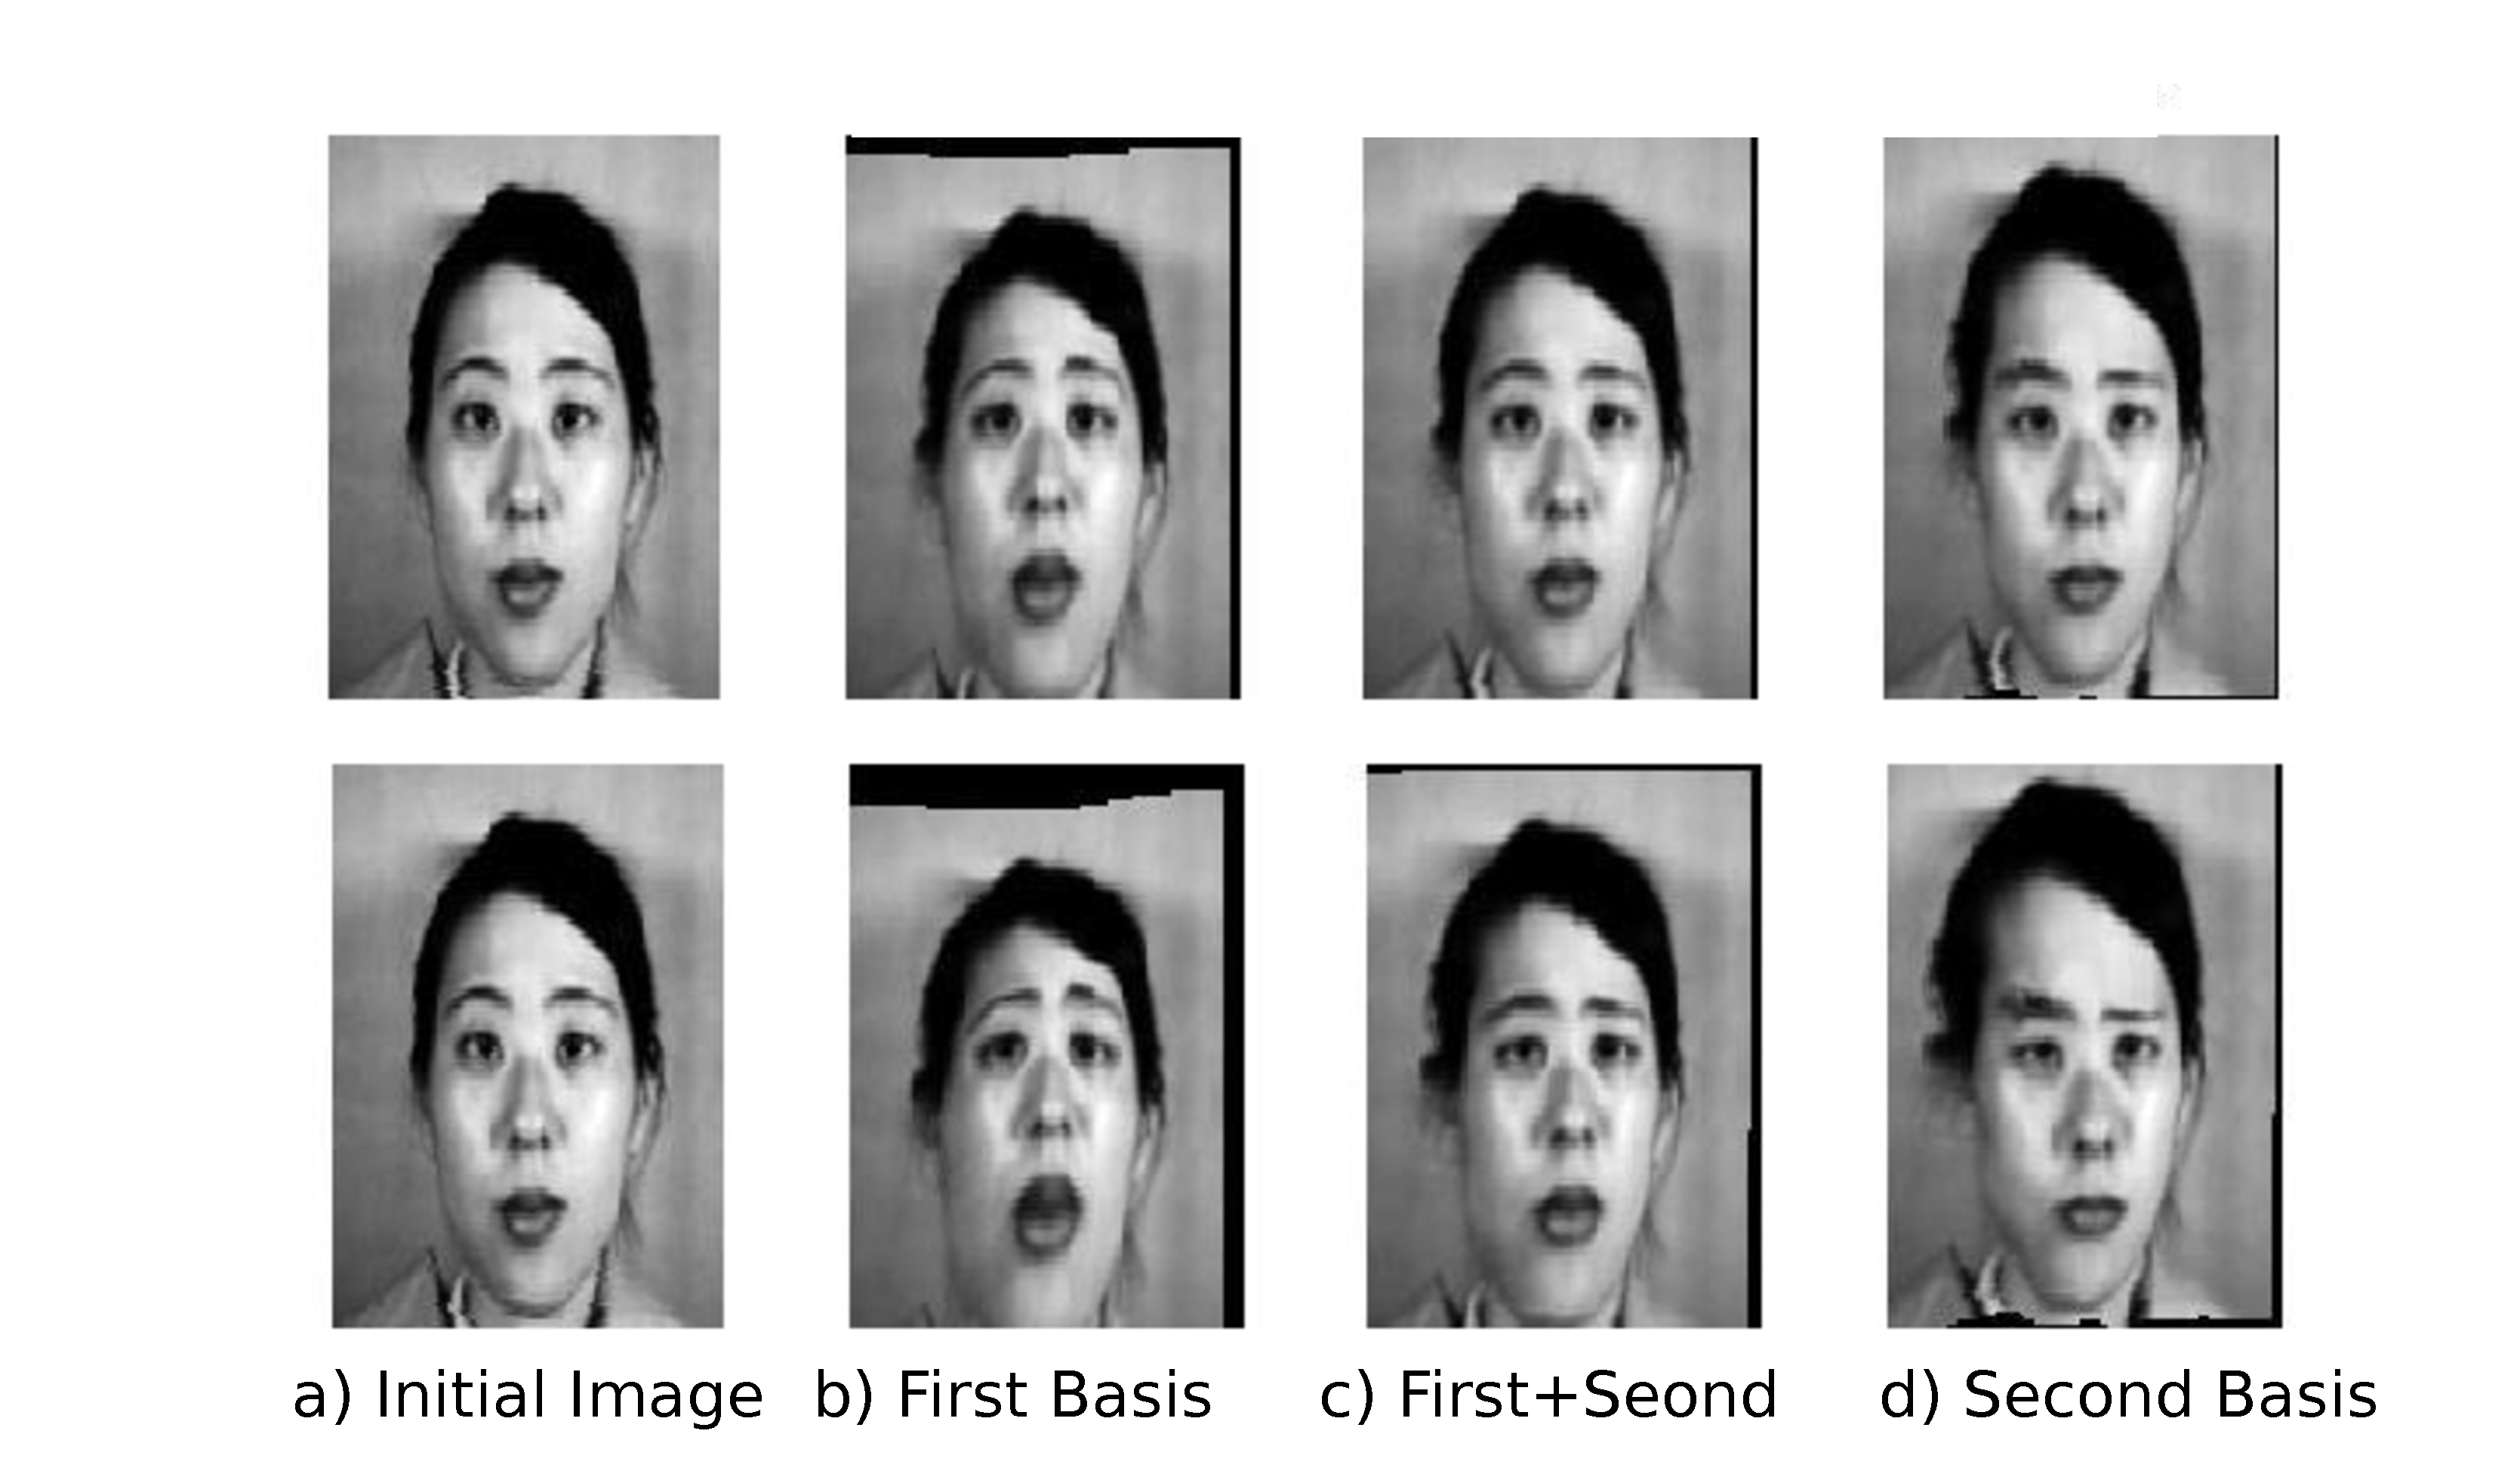
\includegraphics[height=0.6\columnwidth]{figs/V2.pdf}
    \caption{Two intermediate frames from the second row of the video which shows the synthesized new faces from the neutral face along the parallel transported deformation basis of sad, angry with sad and sad expression}
    \label{fig:v2}
\end{figure}

\subsection{Face Reconstruction with Learned Deformation Basis}
Here, we illustrate the influence of sharing deformation bases via parallel transport. These results supplement section 4.3 where only quantitative comparisons are given. The data set in 4.3 is more extensive, but of low quality, lending itself to quantitative analysis, while the data set here allows for qualitative visual comparison.

We create the training set by randomly sampling half of face images from each female model and we randomly pick three from the rest for each model as the testing set to be reconstructed from the trained manifold.
In the first model, we indepently learn the tagent space around the center face, face image closet to the mean face image, for each female model.
In the second model, we first learn the transport flow between the center faces of these two female models and then learn the tagent space around each center face with parallel transported face images.
For comparison, we take five deformation basis for each model in the first model while we use 10 shared deformation basis in the second model.

In Figure~\ref{fig:v3}, we see that the first model (middle row) does a reasonable job when the test images are close to those in the training, like column 3 and 6. However, due to the lack of the training samples, reconstructed images from the first model barely capture the expression in column 1,4 and 5. On the other hand, the second model (bottom row) better recovers the deformation of the test images. 
\begin{figure}[t]
    \centering
    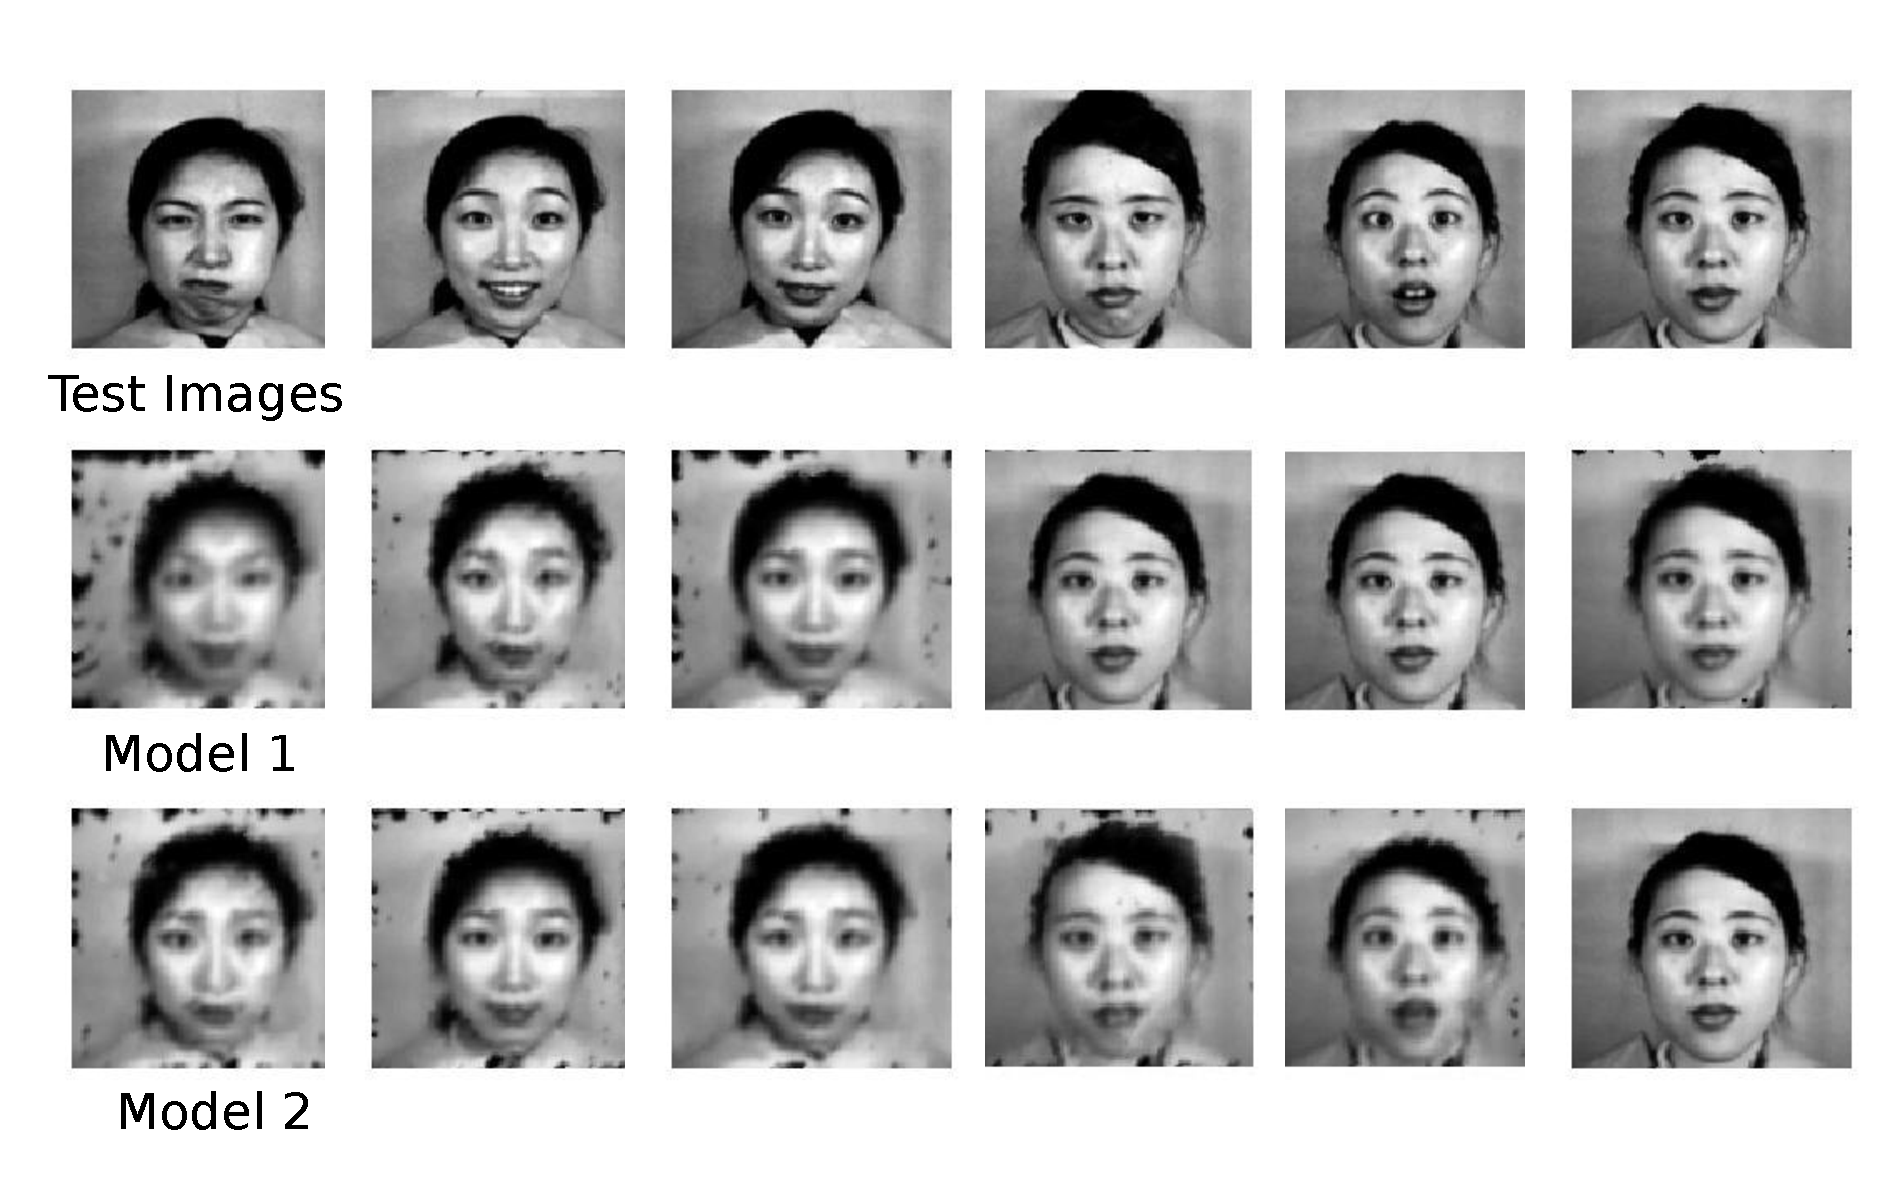
\includegraphics[height=0.6\columnwidth]{figs/V3.pdf}
    \caption{In the top row are the 6 randomly sampled test images to be reconstructed. The middle row shows the reconstructed images from the tagent space independentely learned for the corresponding female model. The bottom row shows the reconstructed images from the tagent space learned with shared deformation basis for the corresponding female model.}
    \label{fig:v3}
\end{figure}


\bibliographystyle{splncs}
\bibliography{sup}

\end{document}
